% !TEX program = pdflatex
% SOICT 2026 submission - Springer LNCS format (single-blind: keep author names).
% Requires the Springer LNCS class `llncs.cls` + `splncs04.bst`.
% Multi-market volatility forecasting model. Figures in docs/paper/figures/.
% MODEL 2026-09-18: XGBoost gamma variants only (XGB / XGB+E / XGB+LG / VolTree).
% LEAK-FIX 2026-09-19: earnings-dependent rows (XGB+E, VolTree) now use the LEAK-FREE expected /
%   point-in-time earnings schedule (release dates predicted from own past cadence, not realized dates):
%   results/gamma_gbm/expected_schedule/leaf_graph_paper_{hose,sp500}_full_h{1,5,10,22}.json
%   (metrics.XGB = XGB+E [full feature set incl. earnings], metrics.XGB+leafgraph = VolTree;
%    + dm + gain_pct + spike_robustness + alpha). GARCH, HAR, GNNHAR, and XGB (endogenous-only) rows
%   are earnings-INDEPENDENT and UNCHANGED.
%   XGB (no-earn) HOSE: results/gamma_gbm/leaf_graph_paper_hose_noearn_h{1,5,10,22}.json (8 folds).
%   XGB (no-earn) SP500: results/gamma_gbm/leaf_graph_paper_sp500_noearn_h{1,5,10,22}.json (8 folds).
%   GARCH MSE/RMSE/MAE added 2026-09-18 (garch_<market>.json metrics; scored over GARCH estimable subset).
% Benchmark rows UNCHANGED: HAR = full_compare_<market>.json + paper_metrics_<market>.json;
%   GNNHAR = gnnhar_<market>.json; GARCH = garch_<market>.json.
% RESTRUCTURE 2026-09-19: reorganized into IMRaD per advisor review. No numbers/cites/cells changed.
%   Fig 1 (fig:arch) moved to 3.3; Fig 2 (fig:eventstudy) moved to 5.1; the three decile/importance
%   figures replaced by one 2x2 panel (fig:diagnostics) in 5.2. tab:detail reduced to the four
%   XGB-family rows (GARCH/HAR/GNNHAR live in tab:summary). Robustness prose relocated to 4.3.
\documentclass[runningheads,a4paper]{llncs}
\usepackage{graphicx}
\graphicspath{{figures/}}
\usepackage{booktabs}
\usepackage{amsmath}
\usepackage{amssymb}
\usepackage{placeins}
\usepackage[utf8]{inputenc}
\usepackage[T1,T5]{fontenc}
\setlength{\emergencystretch}{3em}   % absorb tight justified lines instead of overflowing the margin
\pdfpagewidth=210mm \pdfpageheight=297mm   % A4 physical page (LNCS/CCIS text block unchanged)
% Tighten spacing around floats to fit the page budget (typographic only; no content/number change).
\setlength{\textfloatsep}{5pt plus 1pt minus 1pt}
\setlength{\floatsep}{5pt plus 1pt minus 1pt}
\setlength{\intextsep}{5pt plus 1pt minus 1pt}
\setlength{\abovecaptionskip}{3pt}
\setlength{\belowcaptionskip}{0pt}

\begin{document}

\title{VolTree: Earnings-Aware Gradient Boosting with Leaf-Graph Smoothing for Stock Volatility Forecasting}
\titlerunning{VolTree: Earnings-Aware Gradient Boosting}

\author{Thanh-Quy Nguyen \and Trung-Hoang Le \and Duy-Hoang Tran}
\authorrunning{T.-Q. Nguyen et al.}
\institute{University of Science, Vietnam National University Ho Chi Minh City, Ho Chi Minh City, Vietnam \\ \email{lthoang@hcmus.edu.vn}}

\maketitle
\pagestyle{empty}\thispagestyle{empty}   % SOICT submission: no page numbers

\begin{abstract}
Forecasting daily stock-price volatility---how much a price is likely to swing on a given day---is a core
input to risk management and option pricing. We build a pooled stock-day volatility forecasting model on a
gamma-loss gradient-boosted tree ensemble (XGBoost) over endogenous (own-history) features, and ask where
extra information helps. The endogenous model beats the HAR linear benchmark, a per-stock GARCH, and a learned graph neural network (GNNHAR) on QLIKE at every
horizon. We then study one external signal (earnings) and one cross-sectional denoising mechanism (the leaf
graph) on two structurally different markets. On the S\&P~500, a cadence-estimated earnings feature is a
modest but reliable lever,
cutting QLIKE by a further 2.7 to 3.2\% over the endogenous model at every horizon (Diebold-Mariano
$p<0.001$); on Vietnam's Ho Chi Minh Stock Exchange (HOSE) the earnings lever does not
transfer, localizing the gain to the S\&P~500. Conversely, a leaf-cooccurrence graph that smooths each trading day's
cross-section of forecasts, built from the boosted model's own tree leaves with a validation-fit smoothing
weight, lowers HOSE QLIKE at the one- and five-day horizons by 0.11 to 0.22\% (Diebold-Mariano $p<0.001$); the
gains remain significant after excluding selected market-stress windows. On the S\&P~500 sample the weight
collapses toward zero and the graph has no effect, consistent with a market-specific denoising effect
rather than a universal graph mechanism. VolTree thus stays numerically close to the best market-specific
variant, its two components giving market-specific rather than universally additive gains.
\keywords{Volatility forecasting \and HAR \and Gradient boosting \and Earnings announcements \and Graph smoothing \and Diebold-Mariano.}
\end{abstract}

\section{Introduction}
Financial markets are volatile: prices swing, and the size of those swings, an asset's
\emph{volatility}, is the standard measure of its risk. Because volatility drives option
pricing, capital requirements, and portfolio risk budgeting, forecasting
it accurately is a long-standing problem in financial econometrics~\cite{corsi2009}. Volatility is
not observed directly; it is estimated from prices, so any forecast is a forecast of an estimate. We
target the daily \emph{Parkinson estimator}~\cite{parkinson1980}, which gauges a day's variance from
its high-low price range and uses more of the day's information than a close-to-close measure; the
forecasting target is therefore a variance (a squared quantity), not a standard deviation.

The standard linear approach is the Heterogeneous Autoregressive (HAR) family~\cite{corsi2009}, which predicts
tomorrow's volatility from its own daily, weekly, and monthly averages---deliberately simple yet hard to
beat. We build a stronger pooled stock-day gamma-loss XGBoost ensemble on top of it and ask what extra
information helps, also training a graph neural network on the HAR features~\cite{gnnhar2024} as a
learned-model reference under the same protocol.

On top of this we study one external earnings signal~\cite{patell1981} and one cross-sectional denoising
mechanism under a leakage-controlled walk-forward protocol scored on the quasi-likelihood (QLIKE) loss with date-clustered
Diebold-Mariano tests. We call the full pipeline---endogenous XGBoost with the earnings block and
leaf-graph smoothing---VolTree, with three main findings. First, the pooled endogenous XGBoost
model is a strong, transparent baseline that beats HAR, a per-stock GARCH, and the learned GNNHAR on QLIKE
at every horizon. Second, a cadence-estimated earnings feature is a modest but reliable lever on the
S\&P~500, cutting QLIKE by a further 2.7 to 3.2\% at every horizon (Diebold-Mariano $p<0.001$); on
HOSE-listed Vietnamese stocks it does not transfer, localizing the gain to the S\&P~500. Third, a leaf-cooccurrence
graph that denoises each trading day's cross-section lowers HOSE QLIKE at the one- and five-day horizons
(Diebold-Mariano-significant, still significant after excluding market-stress windows) yet self-disables on
the S\&P~500 sample, a market-specific rather than universal benefit.

\section{Related Work}

\subsection{Statistical Volatility Forecasting}
The classical approach models conditional variance parametrically: Autoregressive Conditional Heteroskedasticity (ARCH)~\cite{engle1982} and its
generalization, Generalized ARCH (GARCH)~\cite{bollerslev1986}, make current variance a function of past squared returns and
variances, and GARCH(1,1) remains a standard benchmark, so we include a per-stock fit. The HAR
model~\cite{corsi2009} regresses realized volatility on its own daily, weekly, and monthly averages, a
deliberately simple yet hard-to-beat linear benchmark. Range-based estimators such as
Parkinson's~\cite{parkinson1980} use a day's high-low range as an efficient variance proxy, exploiting
more information than a close-to-close measure~\cite{alizadeh2002}.

\subsection{Machine-Learning Volatility Forecasting}
Gradient boosting~\cite{friedman2001} and its scalable implementation XGBoost~\cite{chen2016} fit
nonlinear regressors by stagewise addition of trees. Neural and other ML models have also been applied to
realized volatility: Bucci~\cite{bucci2020} evaluates neural architectures and Zhang et
al.~\cite{zhang2024ml} exploit intraday commonality via pooled cross-stock learning. Large-scale evidence
shows nonlinear models do not uniformly beat well-specified linear benchmarks~\cite{branco2024},
reinforcing comparison against HAR; we adopt a pooled gamma-loss boosted-tree model and evaluate it with
QLIKE~\cite{patton2011} and the Diebold-Mariano test~\cite{dm1995}.

\subsection{Graph-Based Financial Forecasting}
Financial dependence has been represented through networks of volatility spillovers and connectedness~\cite{diebold2014},
and graph neural networks have incorporated correlation or spillover structure into realized-volatility
forecasting~\cite{gnnhar2024}; we include the published GNNHAR as a learned baseline. A graph can instead
be derived from the model itself: the random-forest proximity (leaf-incidence) kernel~\cite{rhodes2023}
measures similarity by how often two points share a leaf, which extends to boosted-tree ensembles and
denoises a same-day cross-section rather than fitting a separate network.

\subsection{Earnings Information and Volatility}
Earnings announcements have long been associated with elevated trading activity and price
variability~\cite{beaver1968,patell1981}, with information content differing across
markets~\cite{defond2007}---a plausible basis for heterogeneous S\&P~500-versus-HOSE responses. Because an
expected release date can be estimated before the forecast origin from the firm's historical reporting
cadence, the distance to the nearest release is a natural predictor, but a leakage-safe design must
distinguish a point-in-time schedule (predicted at the forecast origin) from realized dates known only ex
post. We extend this literature by evaluating a leakage-controlled
scheduled-earnings feature jointly with a tree-derived cross-sectional graph across two markets.


\section{Data and Methodology}

\subsection{Forecasting Problem and Target}
\indent\textbf{Forecasting target.} For ticker $i$ on day $t$ we forecast the daily Parkinson variance
\[ \mathrm{pk}_{i,t}=\frac{[\ln(H_{i,t}/L_{i,t})]^2}{4\ln 2}, \]
estimated from the daily high $H_{i,t}$ and low $L_{i,t}$, at horizons $h\in\{1,5,10,22\}$ (roughly a day,
week, fortnight, month). Every feature is observed at the forecast origin $t$, and each horizon forecasts
the single day $t+h$ rather than a cumulative average. We report QLIKE as the primary
loss~\cite{patton2011}, with MSE, RMSE and MAE; for realized target $y$ and forecast $\hat y$,
\[ L_{\mathrm{QLIKE}}(y,\hat y)=\frac{y}{\hat y}-\log\frac{y}{\hat y}-1. \]

\subsection{Datasets}
\textbf{Data sources.} Daily open-high-low-close-volume (OHLCV) data for the 497 S\&P~500 tickers are obtained from Yahoo Finance; the 405 HOSE
tickers are from \texttt{vnstock}, a Vietnamese market-data feed, with each ticker's full daily history
crawled from its listing. The Parkinson target and all endogenous features derive from daily high, low,
and close prices. We use daily OHLC rather than intraday data primarily because daily
open-high-low-close is freely and readily available for both markets at no cost, whereas minute-level
histories are paid or vendor-restricted for the S\&P~500 and largely unavailable for HOSE; moreover, the
range-based Parkinson estimator recovers a day's intraday range from the freely available high and low, so
little information is lost by staying at daily frequency. Earnings dates and their
provenance (Yahoo Finance for the S\&P~500; the State
Securities Commission portal plus a \texttt{vnstock} news feed for HOSE) are detailed in the Limitations.
On both markets, headline forecasts use only a point-in-time cadence-based expected schedule constructed
from prior releases; realized (ex-post) dates are used solely for the event study and upper-bound analysis
(Section~\ref{sec:robust}), never as future-known forecast inputs.

\subsection{VolTree Model}\label{sec:voltree}
\textbf{Model.} The forecasting model is a pooled stock-day gamma-loss gradient-boosted tree
ensemble~\cite{friedman2001} (XGBoost~\cite{chen2016} with the \texttt{reg:gamma} objective, whose
deviance is proportional to QLIKE up to a constant (twice $L_{\mathrm{QLIKE}}$ in the equation above); full configuration in the experimental protocol
below). For each market and horizon a single pooled model is fitted to all training stock-day
observations, so all same-day tickers are routed through the same trees, making their leaf-index vectors
directly comparable. The endogenous feature vector is $\mathbb{R}^8$: three HAR lags~\cite{corsi2009} and
five log-volatility momentum terms. An external earnings block adds $\mathbb{R}^4$ of cadence-estimated
earnings features, chiefly the distance from the forecast target to the nearest release, and a
per-day leaf-cooccurrence graph then smooths the forecasts across each day's cross-section
(Figure~\ref{fig:arch}: features $\rightarrow$ gamma-XGBoost $\rightarrow$ leaf similarity $\rightarrow$
graph smoothing $\rightarrow$ forecast).

The ablation design isolates each component through four variants: \textbf{XGB} uses the endogenous
block only; \textbf{XGB+E} adds the earnings block; \textbf{XGB+LG} adds leaf-graph smoothing to the
endogenous model (no earnings, isolating the graph); and \textbf{VolTree}, the full proposed model,
adds both the earnings block and leaf-graph smoothing. VolTree uses both components; the ablation
quantifies each one's contribution, which is market-specific.

\begin{figure}[t]
\centering
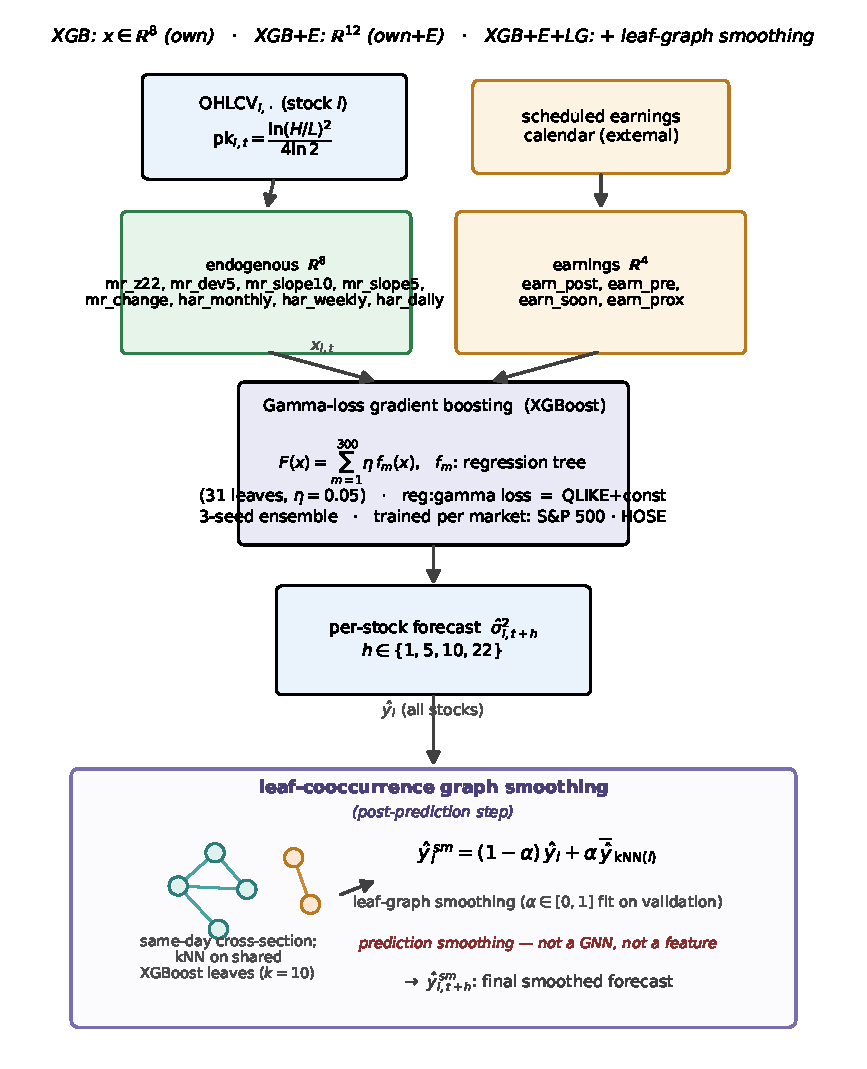
\includegraphics[width=0.62\textwidth]{fig_architecture.pdf}
\caption{VolTree architecture. Endogenous features ($\mathbb{R}^8$) and a cadence-estimated
earnings block ($\mathbb{R}^4$) feed a gamma-loss gradient-boosted tree ensemble (XGBoost);
a per-day leaf-cooccurrence graph then smooths the horizon-specific Parkinson-variance forecast across
the cross-section.}
\label{fig:arch}
\end{figure}
\FloatBarrier

\subsection{Competing Baselines}

\textbf{Baselines.} HAR~\cite{corsi2009} fits three endogenous lags by ordinary least squares (OLS). GARCH is a per-stock
GARCH(1,1) on daily returns.
GNNHAR~\cite{gnnhar2024} is a learned graph neural network over the three HAR lags. For each fold, the
adjacency is a top-10 nearest-neighbour graph built from Pearson correlations of log Parkinson variance over
the training window; only positive correlations are retained, self-correlations are excluded, and each
node's neighbour weights are row-normalized to sum to one. The graph is frozen for validation and test (no
test-window data enters its construction). The network has two graph-convolution layers (hidden width 9),
trained with Adam (learning rate $10^{-3}$, weight decay $10^{-5}$, gradient clipping at 1.0) for at least
20 and at most 120 epochs with early stopping on validation QLIKE (patience 15), run as a three-seed
ensemble; we report the validation-selected variant, with remaining settings following the published
implementation. The XGBoost hyperparameters were pre-specified (not tuned per fold).
All baselines share the XGBoost model's target, protocol, and positivity floor. The XGB, XGB+E, and XGB+LG variants (Section~\ref{sec:voltree}) are ablations of VolTree, not
external baselines.

\subsection{Feature Construction}
\textbf{Endogenous features (8 features, used by XGB).} Every endogenous feature is observable at the
forecast origin $t$. The three HAR lags capture short, medium, and long memory of realized variance
over one day, one trading week (5 trading days), and one trading month (22 days):
\begin{align}
\mathrm{har\_daily} &= \mathrm{pk}_{i,t}, &
\mathrm{har\_weekly} &= \frac{1}{5}\sum_{k=0}^{4}\mathrm{pk}_{i,t-k},\\
\mathrm{har\_monthly} &= \frac{1}{22}\sum_{k=0}^{21}\mathrm{pk}_{i,t-k}. &&
\end{align}
Five log-volatility momentum terms, built on $\ell_{i,t}=\ln(\max(\mathrm{pk}_{i,t},\varepsilon))$ with
$\varepsilon=10^{-8}$, encode recent trend, multi-scale slope, deviation from the recent mean, and a
standardized 22-day level:
\begin{align}
\mathrm{mr\_change} &= \ell_{i,t}-\ell_{i,t-1}, &
\mathrm{mr\_slope5} &= \frac{\ell_{i,t}-\ell_{i,t-5}}{5},\\
\mathrm{mr\_slope10} &= \frac{\ell_{i,t}-\ell_{i,t-10}}{10}, &
\mathrm{mr\_dev5} &= \ell_{i,t}-\frac{1}{5}\sum_{k=0}^{4}\ell_{i,t-k},\\
\mathrm{mr\_z22} &= \frac{\ell_{i,t}-\mu_{22}(\ell_i)}{\sigma_{22}(\ell_i)+\varepsilon}. &&
\end{align}
where $\mu_{22},\sigma_{22}$ are the trailing 22-day mean and standard deviation of $\ell_i$, together
summarizing the stock's short-run acceleration and regime level.

\textbf{Cadence-estimated earnings features (4 features, used by XGB+E).} Each earnings feature is evaluated
at the target day $t+h$ from a cadence-estimated earnings schedule; any release between $t$ and $t+h$ that
the feature uses is a predicted (origin-time) date, never a realized future date. For the headline results
the release date is a point-in-time estimate predicted at the forecast origin from the firm's own past
cadence: the next date is
\[ \hat d_{i,q+1} = d_{i,q} + \operatorname{median}_{j\le q-1}\left(d_{i,j+1}-d_{i,j}\right), \]
the previous release $d_{i,q}$ plus the median of the strictly-prior inter-release gaps in calendar days,
where $q$ indexes ticker $i$'s successive releases and $j$ runs over its prior inter-release gaps.
Before three releases have been observed for a ticker, its four earnings features are set to zero. This is a
causal cadence-based expected schedule that is leakage-safe with respect to the evaluated forecast origins,
since it uses only releases observed before each origin (only inter-release gaps strictly before each event
enter; a caveat quantified in the Limitations); using realized dates instead yields an optimistic upper bound
(Section~\ref{sec:robust}). Let $\mathrm{nxt}$ be the calendar days from $t+h$ to
the next announcement, $\mathrm{prv}$ the calendar days since the previous, and
$\mathrm{dist}=\min(\mathrm{nxt},\mathrm{prv})$:
\begin{align}
\mathrm{earn\_prox} &= \max\!\Big(0,\,1-\tfrac{\mathrm{dist}}{5}\Big), &
\mathrm{earn\_soon} &= \mathbf{1}[\mathrm{dist}\le 3],\\
\mathrm{earn\_pre} &= \max\!\Big(0,\,1-\tfrac{\mathrm{nxt}}{5}\Big), &
\mathrm{earn\_post} &= \max\!\Big(0,\,1-\tfrac{\mathrm{prv}}{10}\Big).
\end{align}
These give a symmetric triangular proximity, a sharp $\pm 3$-day flag, a pre-announcement run-up, and a
longer post-announcement decay. Away from any release all four are zero, so XGB+E reduces to XGB on ordinary
days and activates only in a local window of 5 calendar days before to 10 calendar days after the expected
release (about 15 calendar days).

\subsection{Leaf-Cooccurrence Graph}
\textbf{Leaf-cooccurrence graph.} The graph reuses the fitted booster to denoise its own forecasts across
the same-day cross-section, adding no information beyond the trees. For each stock on each test day we read
the vector of leaf indices assigned by the 300 trees of the fitted booster~\cite{chen2016}; the fraction
of shared leaves between two tickers is a Hamming similarity in $[0,1]$, the boosted-tree analogue of the
random-forest proximity (leaf-incidence) kernel~\cite{rhodes2023}. Within each trading day we build a $k$-nearest-neighbour graph
($k=10$) over that similarity and replace each forecast by
$\hat y_i^{\,\mathrm{LG}}=(1-\alpha)\,\hat y_i+\alpha\,\overline{\hat y}_{\mathcal{N}(i)}$, an unweighted
mean over its neighbours. The graph is a directed $k$-NN---each stock keeps its own $k$ most leaf-similar
same-day peers and is excluded from its own neighbour set---and is not symmetrized. The leaf indices come
from a single fitted booster (the first seed) and the smoothed base forecast is the seed-averaged
prediction; the booster is effectively deterministic, so the two coincide up to negligible seed variation. The weight $\alpha\in[0,1]$ is selected from a grid on the validation slice only,
one value per (market, horizon, fold), and applied once to the test window; XGB+LG and VolTree each fit
their own $\alpha$ on their respective base forecast. The graph is therefore causal, adds no smoothing
when its validation-fit weight $\alpha$ is zero, and introduces no temporal leakage since it spans only the same
day's tickers.

\subsection{Experimental Protocol}
\textbf{Walk-forward evaluation.} Training begins at 2015-01-01, chosen so both markets have a liquid daily
cross-section across the training span---HOSE's broad listing and its earnings coverage are comparatively
recent, so an earlier start (e.g.\ 2000) would leave the Vietnamese panel sparse. We use an expanding-window walk-forward
with eight semi-annual test folds starting 2022-07-01, 2023-01-01, 2023-07-01, 2024-01-01, 2024-07-01,
2025-01-01, 2025-07-01, and 2026-01-01, each spanning the following six months. For fold start $F_k$ and
horizon $h$, training uses all data from 2015-01-01 up to $F_k$ minus an embargo of
$g_h=\lfloor 1.6h\rfloor+5$ calendar days. The embargo grows with the horizon $h$ because a longer-horizon
target reaches further past the fold boundary; removing these rows stops any training row whose
$h$-step-ahead target would fall inside the test window from leaking future information (the
$\lfloor 1.6h\rfloor$ term conservatively covers $h$ trading days and the $+5$ buffers weekends and exchange
holidays). The last 22 training dates are held out as validation. A
separate model is fitted per horizon (direct forecasting: each horizon is predicted from the origin
rather than by iterating a one-step model), so each market has one model per horizon. A fold-horizon is
skipped only if its training block falls below a small per-market row floor; every fold's training block
runs to hundreds of thousands of stock-days and comfortably clears this guard. The leaf-graph weight is selected from
$\alpha\in\{0.0,0.1,\dots,1.0\}$, one per (market, horizon, fold) on the validation slice and applied once
to the test window; the per-day $k$-nearest-neighbour graph uses $k=10$. All fits use training data only,
the test window is read once, and predictions are floored at $10^{-8}$ (so QLIKE, which divides by the
forecast, stays finite) and capped at $1.0$, applied identically to every model so no model gains from
different clipping.

\textbf{Gamma-XGBoost configuration.} Every model uses the \texttt{reg:gamma} objective with 300 boosting
rounds, learning rate 0.05, at most 31 leaves per tree under \texttt{grow\_policy=lossguide}
(\texttt{max\_depth}~0, leaf count controls capacity), L2 penalty $\lambda=1.0$, minimum child weight 20,
\texttt{tree\_method=hist}, and no row/column subsampling
($\texttt{subsample}=\texttt{colsample\_bytree}=1.0$). XGBoost is effectively deterministic under this
no-subsampling configuration; repeated seeds (0, 1, 2, averaged) were used only as an implementation-stability
check, not independent stochastic replications.

\textbf{Metrics and statistical tests.} QLIKE is the primary loss~\cite{patton2011}, with MSE, RMSE and
MAE. We first average loss differentials across stocks within each date to account for contemporaneous
cross-sectional dependence and obtain one loss differential per trading day; the Diebold-Mariano
test~\cite{dm1995} is then applied to this daily loss-differential series. The primary pre-specified comparisons are XGB vs.\ HAR, XGB+E vs.\ XGB, XGB+LG
vs.\ XGB, and VolTree vs.\ its ablation; the rest are secondary.


\section{Empirical Results}

\subsection{Overall Forecasting Performance}
Table~\ref{tab:summary} summarises the headline metrics. Against the three external baselines in
Table~\ref{tab:summary} (GARCH, HAR, GNNHAR), VolTree achieves the lowest QLIKE at every horizon in
both markets. The component ablation (Table~\ref{tab:detail}), however, shows that the market-specific
variants XGB+E (S\&P~500) and XGB+LG (HOSE) attain marginally lower QLIKE than the full model. VolTree also posts the best value on all four metrics
everywhere except the S\&P~500 ten-day horizon, where linear HAR edges it on the squared-error metrics; the
learned GNNHAR never beats it and is worse than even linear HAR at $h1$ on the S\&P~500 (QLIKE 0.375 against
0.370). Table~\ref{tab:detail} then isolates which component drives this.

\begin{table}[!t]
\centering
\caption{External-baseline comparison: three baselines (GARCH, HAR, GNNHAR) versus VolTree at
$h\in\{1,5,10,22\}$ (S\&P~500 left, HOSE right). All four metrics are lower-is-better and are computed as
the mean loss over all test stock-day observations pooled across the eight walk-forward folds, separately
per market and horizon. MSE $\times10^{-6}$, RMSE/MAE $\times10^{-3}$, QLIKE unscaled (as in
Table~\ref{tab:detail}). Bold marks the best (minimum) value in each market--horizon column among these
four models; the component variants are in Table~\ref{tab:detail}.}
\label{tab:summary}
\scriptsize
\setlength{\tabcolsep}{3pt}
\begin{tabular}{ll cccc cccc}
\toprule
& & \multicolumn{4}{c}{\textbf{S\&P~500}} & \multicolumn{4}{c}{\textbf{HOSE}} \\
\cmidrule(lr){3-6}\cmidrule(lr){7-10}
$h$ & Model & MSE & RMSE & MAE & QLIKE & MSE & RMSE & MAE & QLIKE \\
\midrule
1 & GARCH    & 0.796 & 0.892 & 0.327 & 0.465 & 0.630 & 0.794 & 0.487 & 1.656 \\
1 & HAR      & 0.575 & 0.759 & 0.213 & 0.370 & 0.660 & 0.813 & 0.519 & 1.812 \\
1 & GNNHAR   & 0.576 & 0.759 & 0.212 & 0.375 & 0.585 & 0.765 & 0.438 & 1.682 \\
1 & VolTree & \textbf{0.555} & \textbf{0.745} & \textbf{0.207} & \textbf{0.346} & \textbf{0.533} & \textbf{0.730} & \textbf{0.390} & \textbf{1.564} \\
\midrule
5 & GARCH    & 0.789 & 0.888 & 0.343 & 0.508 & 0.703 & 0.838 & 0.537 & 1.740 \\
5 & HAR      & 0.614 & 0.784 & 0.230 & 0.436 & 0.663 & 0.814 & 0.523 & 1.822 \\
5 & GNNHAR   & 0.638 & 0.799 & 0.233 & 0.446 & 0.616 & 0.785 & 0.469 & 1.744 \\
5 & VolTree & \textbf{0.612} & \textbf{0.782} & \textbf{0.225} & \textbf{0.399} & \textbf{0.578} & \textbf{0.760} & \textbf{0.423} & \textbf{1.646} \\
\midrule
10 & GARCH    & 0.757 & 0.870 & 0.349 & 0.522 & 0.734 & 0.857 & 0.565 & 1.782 \\
10 & HAR      & \textbf{0.621} & \textbf{0.788} & 0.236 & 0.461 & 0.666 & 0.816 & 0.525 & 1.828 \\
10 & GNNHAR   & 0.660 & 0.812 & 0.243 & 0.477 & 0.628 & 0.792 & 0.483 & 1.767 \\
10 & VolTree & 0.629 & 0.793 & \textbf{0.231} & \textbf{0.418} & \textbf{0.594} & \textbf{0.771} & \textbf{0.438} & \textbf{1.681} \\
\midrule
22 & GARCH    & 0.739 & 0.860 & 0.363 & 0.544 & 0.788 & 0.888 & 0.606 & 1.837 \\
22 & HAR      & 0.633 & 0.795 & 0.242 & 0.485 & 0.672 & 0.820 & 0.528 & 1.835 \\
22 & GNNHAR   & 0.635 & 0.797 & 0.241 & 0.476 & 0.655 & 0.809 & 0.507 & 1.810 \\
22 & VolTree & \textbf{0.621} & \textbf{0.788} & \textbf{0.234} & \textbf{0.434} & \textbf{0.621} & \textbf{0.788} & \textbf{0.458} & \textbf{1.725} \\
\bottomrule
\end{tabular}
\end{table}

\subsection{Component Ablation}
Table~\ref{tab:detail} isolates the four XGB-family variants. The endogenous XGB already beats HAR and
GARCH on QLIKE at every horizon. On the S\&P~500 the earnings block drives the further improvement---XGB+E
carries the bolded QLIKE in every block---while leaf-graph smoothing self-disables. On HOSE the pattern
reverses: the earnings block is inert (XGB+E indistinguishable from XGB) and the leaf-graph is the only
component that lowers QLIKE, so XGB+LG attains the lowest HOSE QLIKE at every horizon (significantly at $h1$
and $h5$) with VolTree closely tracking it.

\begin{table}[!t]
\centering
\caption{Component ablation of the four XGB-family variants (S\&P~500 left; HOSE
right; walk-forward; seeds averaged as a stability check, not independent replications; all metrics
lower-is-better, aggregated as in Table~\ref{tab:summary}). XGB is endogenous-only, XGB+E adds earnings,
XGB+LG adds leaf-graph smoothing, and VolTree adds both (the full model).
MSE $\times10^{-6}$, RMSE/MAE $\times10^{-3}$, QLIKE unscaled (as in Table~\ref{tab:summary}). Bold marks
the best (minimum) value in each market--horizon column. For QLIKE significance ($^{*}$, $p<0.05$, Section~\ref{sec:robust}): XGB+E
and XGB+LG are each tested against XGB; VolTree is tested against XGB+E and XGB+LG separately. $^{\dagger}$
marks a numerical improvement over XGB that is not statistically significant, and no marker is shown
when the full model does not improve either component. Tests use unrounded losses; baselines are in
Table~\ref{tab:summary}.}
\label{tab:detail}
\scriptsize
\setlength{\tabcolsep}{3pt}
\begin{tabular}{ll cccc cccc}
\toprule
& & \multicolumn{4}{c}{\textbf{S\&P~500}} & \multicolumn{4}{c}{\textbf{HOSE}} \\
\cmidrule(lr){3-6}\cmidrule(lr){7-10}
$h$ & Model & MSE & RMSE & MAE & QLIKE & MSE & RMSE & MAE & QLIKE \\
\midrule
% Table 2 ablation rows: QLIKE to 4 dp; bold = numerical column min; ^* = DM-significant improvement over
% the ablation base (earnings for XGB+E, leaf-graph for XGB+LG/VolTree); ^\dagger = numerical min, not sig.
% Source: leaf_graph_paper_{mkt}_noearn (XGB, XGB+LG) + expected_schedule/leaf_graph_paper_{mkt}_full (XGB+E, VolTree).
1 & XGB      & 0.558 & 0.747 & 0.209 & 0.3573 & 0.534 & 0.731 & 0.392 & 1.5675 \\
1 & XGB+E    & \textbf{0.554} & \textbf{0.744} & 0.208 & \textbf{0.3457$^{*}$} & 0.534 & 0.731 & 0.392 & 1.5675 \\
1 & XGB+LG   & 0.557 & 0.746 & 0.209 & 0.3573 & 0.534 & \textbf{0.730} & \textbf{0.390} & \textbf{1.5640$^{*}$} \\
1 & VolTree  & 0.555 & 0.745 & \textbf{0.207} & 0.3458 & \textbf{0.533} & \textbf{0.730} & \textbf{0.390} & \textbf{1.5640} \\
\midrule
5 & XGB      & 0.613 & 0.783 & 0.226 & 0.4121 & \textbf{0.578} & \textbf{0.760} & 0.425 & 1.6474 \\
5 & XGB+E    & \textbf{0.611} & \textbf{0.782} & \textbf{0.225} & \textbf{0.3992$^{*}$} & \textbf{0.578} & \textbf{0.760} & 0.425 & 1.6474 \\
5 & XGB+LG   & 0.613 & 0.783 & 0.226 & 0.4122 & \textbf{0.578} & \textbf{0.760} & \textbf{0.423} & \textbf{1.6455$^{*}$} \\
5 & VolTree  & 0.612 & \textbf{0.782} & \textbf{0.225} & 0.3995 & \textbf{0.578} & \textbf{0.760} & \textbf{0.423} & \textbf{1.6455} \\
\midrule
10 & XGB      & 0.631 & 0.794 & 0.232 & 0.4311 & 0.595 & \textbf{0.771} & 0.439 & 1.6816 \\
10 & XGB+E    & \textbf{0.628} & \textbf{0.793} & \textbf{0.231} & \textbf{0.4182$^{*}$} & 0.595 & \textbf{0.771} & 0.439 & 1.6818 \\
10 & XGB+LG   & 0.631 & 0.794 & 0.232 & 0.4312 & \textbf{0.594} & \textbf{0.771} & \textbf{0.438} & \textbf{1.6814$^{\dagger}$} \\
10 & VolTree  & 0.629 & \textbf{0.793} & \textbf{0.231} & 0.4184 & \textbf{0.594} & \textbf{0.771} & \textbf{0.438} & 1.6815 \\
\midrule
22 & XGB      & 0.623 & 0.789 & 0.236 & 0.4459 & \textbf{0.621} & \textbf{0.788} & 0.459 & 1.7251 \\
22 & XGB+E    & \textbf{0.621} & \textbf{0.788} & \textbf{0.234} & \textbf{0.4340$^{*}$} & \textbf{0.621} & \textbf{0.788} & 0.459 & 1.7253 \\
22 & XGB+LG   & 0.623 & 0.789 & 0.236 & 0.4459 & \textbf{0.621} & \textbf{0.788} & \textbf{0.458} & \textbf{1.7250$^{\dagger}$} \\
22 & VolTree  & \textbf{0.621} & \textbf{0.788} & \textbf{0.234} & \textbf{0.4340} & \textbf{0.621} & \textbf{0.788} & \textbf{0.458} & 1.7252 \\
\bottomrule
\end{tabular}
\end{table}

\subsection{Statistical and Robustness Analysis}\label{sec:robust}
All Diebold-Mariano tests for the emphasized component comparisons---the S\&P~500 earnings increment and
the HOSE leaf-graph gains at $h1$ and $h5$---yield $p<0.001$; Table~\ref{tab:detail} uses a $p<0.05$ marker
for compactness.

\textbf{Leaf-graph significance on HOSE.} Smoothing the forecasts over the per-day leaf-cooccurrence graph
lowers HOSE QLIKE relative to the unsmoothed model at the one- and five-day
horizons: the gain is 0.22\% ($h1$, DM $p<0.001$) and 0.11\% ($h5$, DM $p<0.001$), and is not
significant at $h10$ (0.02\%, DM $p=0.48$) or $h22$ (0.01\%, DM $p=0.85$).
% gains + DM: expected_schedule/leaf_graph_paper_hose_full_h{1,5,10,22}.json gain_pct / dm.XGB+leafgraph_vs_XGB
The lever is endogenous denoising, not earnings: the no-earnings ablation XGB+LG (leaf-graph on the
endogenous model, Table~\ref{tab:detail}) gains 0.22\% at $h1$ and 0.12\% at $h5$ (both DM $p<0.001$) over
XGB, matching the rounded VolTree values at $h1$ and $h5$ because the HOSE earnings block is effectively
inert.
% no-earn: leaf_graph_paper_hose_noearn_h{1,5}.json gain_pct / dm
The weight $\alpha$ varies by fold: the mean validation-selected $\alpha$ ranges 0.22 to 0.35 across
horizons, per-fold values span 0.0 to 0.8 (the median selected weight is about 0.40 at $h1$ and 0.15 to 0.20 across
the longer horizons), so the graph is materially active there. On the S\&P~500 sample the construction has no effect:
the validation-fit weight collapses toward zero (mean $\alpha$ 0.00 to 0.10) and the QLIKE change stays
within 0.07\% and never significant, so the validation-fit weight $\alpha$ stays near zero where validation
does not support additional smoothing.
% SP500 alpha + gains: expected_schedule/leaf_graph_paper_sp500_full_h{1,5,10,22}.json alpha.mean (0.10/0.075/0.0375/0.00) / gain_pct (-0.043/-0.066/-0.040/0.00) / dm

\textbf{Spike robustness.} The HOSE gains survive the spike-robustness screen: excluding the within-test
stress windows---the 2022 drawdown (2022-07-01 to 2022-12-30) and the April 2025 U.S.
tariff-announcement window (2025-04-01 to 2025-04-30), a market-wide shock relevant to both markets
(57{,}466 excluded observations)---the leaf-graph still beats the unsmoothed model at
$h1$ and $h5$ (ex-spike gain 0.23\% and 0.09\%; DM $p<0.001$).
% ex-spike: expected_schedule/leaf_graph_paper_hose_full_h{1,5}.json spike_robustness.gain_pct_ex_spike (0.2298/0.0932) / dm_p_ex_spike (6.7e-4/8.1e-4)
The endogenous advantage is likewise a calm-market property: the endogenous model beats HAR at every
horizon by about 13\% on QLIKE (at $h1$, 1.568 against 1.812, a 13.5\% gain), and this persists after
excluding the within-test stress windows---the 2022 drawdown (2022-07-01 to 2022-12-30) and the April 2025
U.S. tariff-announcement window---so it is not an artifact of a few crisis days.
% XGB vs HAR: expected_schedule/leaf_graph_paper_hose_full_h1.json metrics.XGB (1.56753) vs full_compare_hose.json HAR (1.81169) = 13.5%

\textbf{Realized-date upper bound.} Under the point-in-time schedule the
incremental S\&P~500 earnings gain is 2.7 to 3.2\% over the endogenous model, DM-significant at every
horizon ($h1$ 3.2\%, $h5$ 3.1\%, $h10$ 3.0\%, $h22$ 2.7\%; all $p<0.001$). Using realized dates instead
raises the measured gain to 8.7 to 11.2\% (per horizon 11.2/10.0/9.1/8.7\%; 14 to 16\% over HAR; not
tabulated), an optimistic upper bound because the realized date is unknown at the forecast origin.
% Headline = leak-free expected schedule: incremental earnings h1 3.24/h5 3.13/h10 3.00/h22 2.68% (leaf_graph_paper_sp500_{noearn,full}_h*.json).
% Earnings DM (headline pipeline, XGBoost): expected_schedule/earnings_dm_sp500.json earn_gain_pct 3.24/3.13/3.00/2.68 dm_p 1.0e-25/3.7e-7/8.2e-5/3.6e-6 (all <1e-3). Upper bound (actual dates, XGBoost): leaf_graph_paper_sp500_{noearn,full}_h* = 11.16/9.98/9.13/8.71% over noearn (14-16% over HAR).


\section{Analysis and Discussion}

\subsection{Earnings Effects on the S\&P 500}\label{sec:earn}
The ex-post event study (Fig.~\ref{fig:eventstudy}) shows that realized S\&P~500 earnings announcements are
associated with a pronounced announcement-day volatility spike---the median variance rises to about 2.75
times baseline---whereas on HOSE it stays flat; this motivates the cadence-estimated proximity features used
at forecast time.

\begin{figure}[t]
\centering
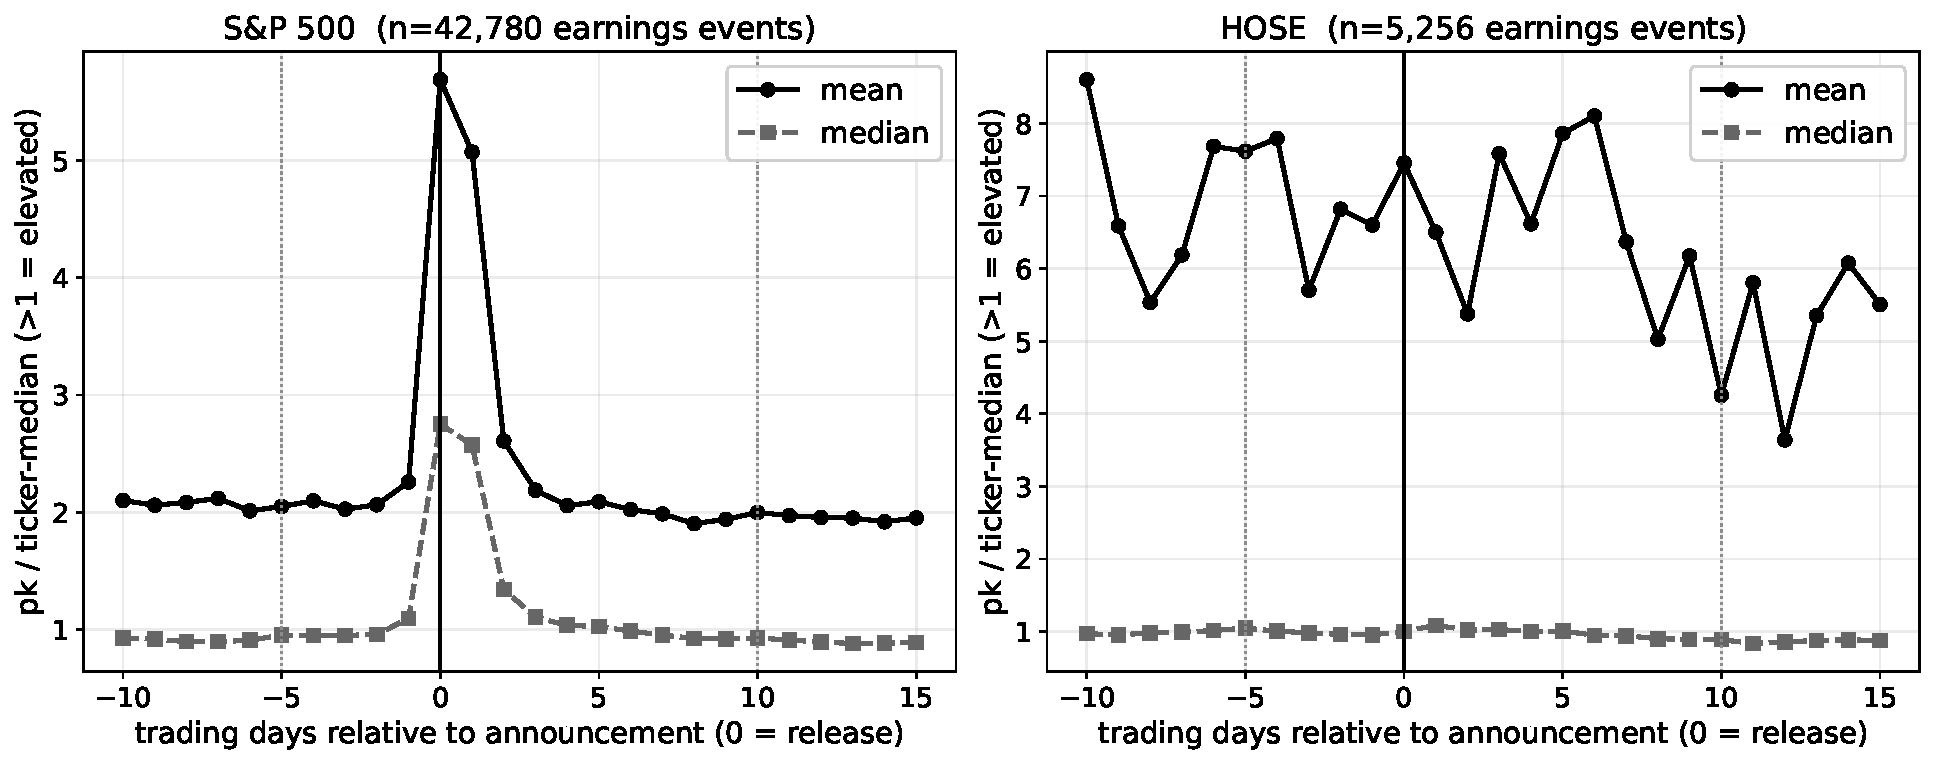
\includegraphics[width=0.50\linewidth]{fig_earnings_event_study.pdf}
\caption{Ex-post event study: mean and median realized Parkinson variance, normalised by each ticker's
median, around realized earnings dates (panel-specific $y$-scales; S\&P~500 $n{=}42{,}780$ announcement
events, HOSE $n{=}5{,}256$ announcement events). The S\&P~500 median rises to about 2.75 times baseline on the announcement day and returns
within a week; the HOSE median stays near one at every offset. This pattern is consistent with the stronger forecasting contribution of the earnings feature
on the S\&P~500.}
\label{fig:eventstudy}
\end{figure}

\textbf{The earnings feature is the lever.} In Table~\ref{tab:detail}, XGB+E posts the lowest S\&P~500
QLIKE at every horizon, gaining 6.5 to 10.6\% over HAR ($h1$ 6.5\%, $h5$ 8.5\%, $h10$ 9.4\%, $h22$ 10.6\%),
% XGB+E QLIKE (leaf_graph_paper_sp500_full_h*.json) vs HAR (full_compare_sp500.json)
decomposing into an endogenous-nonlinearity component (XGB over HAR: $h1$ 3.4\%, $h5$ 5.6\%, $h10$ 6.6\%,
$h22$ 8.1\%, the horizon-growing share) and an incremental earnings component (XGB+E over XGB: $h1$ 3.2\%,
$h5$ 3.1\%, $h10$ 3.0\%, $h22$ 2.7\%). Earnings are a reliable but modest lever---DM-significant at every
horizon ($p<0.001$)---while the endogenous model does most of the work.
% incremental earnings (leak-free expected schedule) = (XGB_noearn - XGB+E)/XGB_noearn: leaf_graph_paper_sp500_noearn_h*.json metrics.XGB (0.35726/0.41210/0.43112/0.44595) vs expected_schedule/leaf_graph_paper_sp500_full_h*.json metrics.XGB (0.34569/0.39921/0.41819/0.43401) = 3.24/3.13/3.00/2.68%
% earnings-increment DM (point-in-time cadence, headline XGBoost pipeline): results/gamma_gbm/expected_schedule/earnings_dm_sp500.json dm_p all <0.001 (~3% QLIKE gain over ~500k obs)

\subsection{Cross-Market Analysis: S\&P 500 versus HOSE}\label{sec:hose}
\textbf{The endogenous model wins on HOSE too.} On HOSE under the identical protocol
(390{,}577 to 399{,}040 stock-day observations per horizon), the endogenous XGBoost model is again the
DM-verified best non-graph model at every horizon, HAR trails widely, and the earnings feature does not
improve it, consistent with the flat HOSE event study. The learned GNNHAR again loses at
every horizon (QLIKE worse by 4.9 to 7.3\%, DM $p<0.001$).
% GNNHAR (gnnhar_hose.json) vs XGB+E (leaf_graph_paper_hose_full_h{1,22}.json): (1.68233-1.56753)/1.56753=7.3%, (1.81018-1.72533)/1.72533=4.9%

\textbf{Earnings does not transfer to Vietnam.} Using the point-in-time expected schedule, XGB+E is within
0.02\% of XGB at every horizon. The HOSE earnings event study (Fig.~\ref{fig:eventstudy}) shows no
announcement-day spike, unlike the S\&P~500; one possible explanation, not directly tested here, is that
Vietnam's daily price limits may delay or dampen the announcement-day adjustment. The result holds in the
well-covered 2025-2026 folds, so it does not rest on missing dates.

\subsection{Practical Interpretation}
No external feature is universally useful for daily volatility forecasting: earnings help the
strong-announcement S\&P~500 but not HOSE (where price limits may mute the response), while
leaf-based smoothing helps the HOSE cross-section but self-disables on the S\&P~500 sample. A strong
endogenous model plus a market-appropriate external signal is what matters.

\FloatBarrier
\section{Limitations}
\noindent\textbf{Earnings archive.} The S\&P~500 dates are Yahoo Finance announcement dates (via
yfinance), a single source capped at 100 events per ticker, so older quarters are truncated; using present
constituents may also carry survivorship bias.

\noindent\textbf{Vietnam coverage.} The HOSE dates are real disclosure dates merged from two crawlers---the
State Securities Commission portal (dense only for 2025-01 through 2026-09) and a sparse 2016-2026 vnstock
news feed covering roughly 218 tickers---with no imputation. Unlike the S\&P~500, each HOSE quarter emits
several distinct filings (parent, consolidated, and combined statements across quarterly, semi-annual, and
annual periods); taking the earliest disclosure per fiscal quarter gives an own-cadence schedule whose
median prediction error is 3 days, close to the 2 days on the S\&P~500, though with a heavier tail from a
minority of firms with irregular filing gaps. The lever's failure to transfer therefore reflects the muted
announcement-day volatility response on HOSE (Fig.~\ref{fig:eventstudy}) rather than a noisy schedule;
given the limited disclosure coverage we still claim only no incremental earnings value under the available
HOSE dates, not a definitive full-history null.

\noindent\textbf{Leaf-graph scope.} The graph is a small market-specific lever---cross-sectional denoising
of the model's own forecasts, not new outside information---whose gains, though significant, are a few
tenths of a percent and associational rather than causal.

\noindent\textbf{Design and evaluation caveats.} The two markets use different constituent construction
(present-membership S\&P~500 versus listing-based HOSE); the leaf-graph weight $\alpha$ is selected on a short 22-date validation slice; no explicit
liquidity statistic supports the market interpretation, which is therefore descriptive; and the XGBoost
seeds are not independent replications, as the model is effectively deterministic under the no-subsampling
configuration. The spike-robustness stress windows were pre-specified (fixed before evaluation) and lie
within the 2022-onward test period. The GNNHAR comparison reflects the validation-selected variant.
Individual $p$-values warrant multiple-comparison caution beyond the primary tests. Genuine point-in-time
earnings calendars were unavailable, so the earnings gain is bracketed by the cadence-based estimate and a
realized-date upper bound. The analysis covers two markets, and its conclusions are limited to daily
OHLC-based Parkinson variance and may not transfer to volatility measured from intraday prices or implied by option prices.

\section{Conclusion}
We built VolTree, a pooled stock-day gamma-loss XGBoost model over endogenous features, extended by a
cadence-estimated earnings block and a leaf-cooccurrence graph that smooths each day's cross-section. The
endogenous model beats the HAR and GARCH benchmarks and a learned GNNHAR on QLIKE at every horizon. On the
S\&P~500 the earnings feature cuts QLIKE by a further
2.7 to 3.2\%; replicated on HOSE-listed Vietnamese stocks the endogenous model again wins, but the earnings lever
does not transfer while the leaf-cooccurrence graph becomes a small but significant short-horizon lever that
self-disables on the S\&P~500 sample. VolTree thus stays numerically close to the best
market-specific variant in each market, with earnings and leaf-based smoothing giving distinct,
market-specific rather than universally additive gains. Future work should extend beyond two markets and to
volatility measured from intraday prices or implied by option prices.

\begin{thebibliography}{99}
\bibitem{corsi2009} Corsi, F.: A simple approximate long-memory model of realized volatility. J. Financial Econometrics \textbf{7}(2), 174--196 (2009)
\bibitem{engle1982} Engle, R.F.: Autoregressive conditional heteroscedasticity with estimates of the variance of United Kingdom inflation. Econometrica \textbf{50}(4), 987--1007 (1982)
\bibitem{bollerslev1986} Bollerslev, T.: Generalized autoregressive conditional heteroskedasticity. J. Econometrics \textbf{31}(3), 307--327 (1986)
\bibitem{parkinson1980} Parkinson, M.: The extreme value method for estimating the variance of the rate of return. J. Business \textbf{53}(1), 61--65 (1980)
\bibitem{patton2011} Patton, A.J.: Volatility forecast comparison using imperfect volatility proxies. J. Econometrics \textbf{160}(1), 246--256 (2011)
\bibitem{dm1995} Diebold, F.X., Mariano, R.S.: Comparing predictive accuracy. J. Business \& Economic Statistics \textbf{13}(3), 253--263 (1995)
\bibitem{friedman2001} Friedman, J.H.: Greedy function approximation: a gradient boosting machine. Annals of Statistics \textbf{29}(5), 1189--1232 (2001)
\bibitem{patell1981} Patell, J.M., Wolfson, M.A.: The ex ante and ex post price effects of quarterly earnings announcements reflected in option and stock prices. J. Accounting Research \textbf{19}(2), 434--458 (1981)
\bibitem{gnnhar2024} Zhang, C., Pu, X., Cucuringu, M., Dong, X.: Forecasting realized volatility with spillover effects: perspectives from graph neural networks. Int. J. Forecasting \textbf{41}(1), 377--397 (2025)
\bibitem{chen2016} Chen, T., Guestrin, C.: XGBoost: a scalable tree boosting system. In: Proceedings of the 22nd ACM SIGKDD International Conference on Knowledge Discovery and Data Mining, pp. 785--794 (2016)
\bibitem{rhodes2023} Rhodes, J.S., Cutler, A., Moon, K.R.: Geometry- and accuracy-preserving random forest proximities. IEEE Trans. Pattern Analysis and Machine Intelligence \textbf{45}(9), 10947--10959 (2023)
\bibitem{bucci2020} Bucci, A.: Realized volatility forecasting with neural networks. J. Financial Econometrics \textbf{18}(3), 502--531 (2020)
\bibitem{zhang2024ml} Zhang, C., Zhang, Y., Cucuringu, M., Qian, Z.: Volatility forecasting with machine learning and intraday commonality. J. Financial Econometrics \textbf{22}(2), 492--530 (2024)
\bibitem{branco2024} Branco, R.R., Rubesam, A., Zevallos, M.: Forecasting realized volatility: does anything beat linear models? J. Empirical Finance \textbf{78}, 101524 (2024)
\bibitem{beaver1968} Beaver, W.H.: The information content of annual earnings announcements. J. Accounting Research \textbf{6}, 67--92 (1968)
\bibitem{defond2007} DeFond, M., Hung, M., Trezevant, R.: Investor protection and the information content of annual earnings announcements: international evidence. J. Accounting and Economics \textbf{43}(1), 37--67 (2007)
\bibitem{alizadeh2002} Alizadeh, S., Brandt, M.W., Diebold, F.X.: Range-based estimation of stochastic volatility models. J. Finance \textbf{57}(3), 1047--1091 (2002)
\bibitem{diebold2014} Diebold, F.X., Yilmaz, K.: On the network topology of variance decompositions: measuring the connectedness of financial firms. J. Econometrics \textbf{182}(1), 119--134 (2014)
\end{thebibliography}

\end{document}
